\subsection{Encryptors}

Public-key encryption involves certain concepts: public and private keys, plain- and ciphertexts. In the adapted ElGamal encryption,
a public key is a \verb+Point+, a private key is a \verb+BigInteger+, and both plaintext and ciphertext are byte-strings. Many
cryptographic implementations (BouncyCastle included) represent all of these concepts as such: their primitive representations.

This practice, however, is not recommendable in an Object-Oriented implementation: Objects are concepts, and there is a very obvious
distinction between the primitive (curve-level) and abstract (encryption-level) constructs. Where curves know about points, encryption
algorithms know about keys. Neither of these should know about byte-strings.

\begin{figure}[htb]
    \begin{tabular}{|p{\textwidth}|}
        \hline
        \textbf{OpenECC} \\
        \hline
        \texttt{Ciphertext Encrypt(PublicKey pub, Plaintext m)} \\
        \texttt{Plaintext Decrypt(PrivateKey priv, Ciphertext c)} \\
        \hline
    \end{tabular}
    
    \begin{tabular}{|p{\textwidth}|}
        \hline
        \textbf{Traditional} \\
        \hline
        \texttt{byte[] Encrypt(Point q, byte[] m)} \\
        \texttt{byte[] Decrypt(BigInteger d, byte[] c)} \\
        \hline
    \end{tabular}

    \caption{The OpenECC type of method signature makes the intention clear, whereas some confusion may exist with the alternative
        (but more traditional) version. For example, what is the point \(q\) -- or the integer \(d\) -- supposed to represent?}
    \label{fig:encryptor_method_signatures}
\end{figure}

The \verb+OpenECC.Encryption.Core+ library implements small wrappers around these concepts, making the interfaces of both encoders and
encryptors easier to read (see Figure \ref{fig:encryptor_method_signatures}). In addition, wrapping the data in classes has made it
possible to add easy conversions to appropriate types, allowing, for example, \verb+Plaintext+s to be represented as \verb+string+s with
a single call: \verb+m.ToString()+.

\begin{figure}[htb]
	\centering
	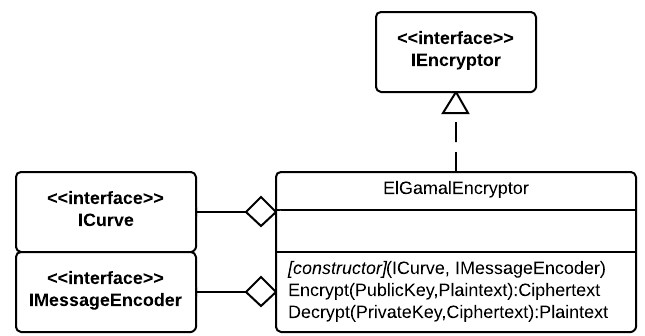
\includegraphics[width=0.7\textwidth]{implementation/encryptors}
	\caption{The only encryptors currently supported rely on public-key cryptography. Like encoders, the encryptors have their state set
		in their constructors, and provide a simple interface for the encryption (\((PublicKey,Plaintext) \to Ciphertext\)) and decryption
		(\((PrivateKey,Ciphertext) \to Plaintext\)) operations themselves. In addition, the encryptors must provide a way to generate a
		random key-pair.}
\end{figure}

The use of encryptors, like the use of multipliers and encoders, allows for extensions of the project, by adding new encryption schemes.
As the encryption schemes are the top-level construct, and there are no components that depend on them, it is very much possible to take
advantage of the underlying structure without having a new encryptor living up to the provided interface.

Using the interface, however, allows aggregating projects to change which encryption scheme to use by changing a single line of code (the
line of the constructor of the encryptor).

Whereas the adapted ElGamal scheme relies purely on elliptic curves, some cryptosystems rely on both elliptic curves and more traditional
cryptography. Such systems are called \emph{hybrid} systems, and ECIES (Elliptic Curve Integrated Encryption Scheme) is one of them. This
system has an elliptic curve point as public key and an integer as private key (just like the adapted ElGamal), but relies internally on
AES/Rijndael.\cite{hankerson2010}

This has the advantage of not relying on any encoding, which in turn lifts the limitation on message length. ECIES could be implemented to
fit the current interfaces in the system.